% !TeX root = ../../Book3.tex
% 纲要标题：### 8.3 增长、覆盖和基本群
% 纲要位置：几何学计划纲要.md，第 2411 行。
% 正文状态：初稿；尚未正式审核。

% 纲要内容开始
% 
% * 非紧流形的体积增长
% * 覆盖空间中的体积计数
% * 有限生成子群的增长约束
% * Euclid、双曲及乘积模型
% 
% 纲要内容结束

\section{增长、覆盖和基本群}
\label{g3:sec:0803}

非负 Ricci 曲率给出球体积的上界，但非紧流形中的球也必须不断容纳新的点。将体积比较的球心移向无穷远，可以把这种非紧性变成定量的体积下界。另一方面，在万有覆盖中，同一点的不同提升彼此分离；每个提升周围都放入一个小球，便能用大球体积估计这些提升的数目。这是体积比较与基本群增长之间的联系。

\subsection{非紧流形的体积增长}
\label{g3:subsec:0803:01}

记 \(V_p(R)=\operatorname{Vol}_g B(p,R)\)，并沿用上一节的约定：\(\omega_n\) 是 \(\mathbb R^n\) 中单位球的体积，\(\sigma_{n-1}=n\omega_n\) 是单位球面的面积。由\cref{g3:thm:bishop-gromov}，若 \(\operatorname{Ric}\ge0\)，则 \(V_p(R)/R^n\) 不增。结合小球体积的 Euclid 极限，立即得到 \(V_p(R)\le\omega_nR^n\)。要取得下界，我们先构造一条在任意长时间上都保持最短的测地线。

\begin{definition}\label{g3:def:geodesic-ray}
	设 \((M,g)\) 为光滑黎曼流形。若单位速测地线 \(\gamma:[0,\infty)\to M\) 满足
	\[
		d_g(\gamma(s),\gamma(t))=t-s
		\qquad(0\le s\le t),
	\]
	则称 \(\gamma\) 为一条\term[cedishexian]{测地射线}[geodesic ray]。因此，射线的每个有限子段都实现其端点距离。
\end{definition}

\begin{lemma}\label{g3:lem:complete-noncompact-ray}
	设 \((M,g)\) 为连通、完备、非紧、无边界的有限维光滑黎曼流形。对每个 \(p\in M\)，都存在从 \(p\) 出发的测地射线。
\end{lemma}
\begin{proof}
	由\cref{g3:thm:hopf-rinow}，闭有界集紧。因此 \(M\) 关于 \(p\) 无界，否则 \(M\) 本身就是一个紧的闭有界集。可取 \(q_j\in M\)，使 \(L_j=d_g(p,q_j)\to\infty\)。同一定理给出从 \(p\) 到 \(q_j\) 的单位速最短测地线
	\[
		\gamma_j(t)=\exp_p(tu_j),\qquad
		0\le t\le L_j,\qquad |u_j|=1.
	\]
	单位球面 \(S_pM\subset\mathrm T_pM\) 紧，故取子列后可设 \(u_j\to u\)，其中 \(|u|=1\)。完备性使 \(\gamma(t)=\exp_p(tu)\) 对所有 \(t\ge0\) 有定义；\cref{g3:thm:geodesic-ivp}的初值光滑依赖给出每个固定 \(t\) 处的 \(\gamma_j(t)\to\gamma(t)\)。

	固定 \(0\le s\le t\)。当 \(j\) 足够大时，\(L_j\ge t\)，而最短线的子段仍最短，所以
	\[
		d_g(\gamma_j(s),\gamma_j(t))=t-s.
	\]
	距离函数连续，取极限即得 \(d_g(\gamma(s),\gamma(t))=t-s\)。由于 \(s,t\) 任意，\(\gamma\) 是所需射线。
\end{proof}

\begin{theorem}\label{g3:thm:noncompact-volume-growth}
	设 \((M^n,g)\) 为连通、完备、非紧、光滑无边界黎曼流形，\(n\ge2\)，且 \(\operatorname{Ric}\ge0\)。对任意 \(p\in M\)，有
	\begin{equation}\label{g3:eq:noncompact-linear-volume}
		\frac{V_p(1)}{4n}R
		\le V_p(R)\le\omega_nR^n
		\qquad(R\ge5).
	\end{equation}
	特别地，\(M\) 的总体积无限。
\end{theorem}
\begin{proof}
	上界已由 Bishop--Gromov 比较及 \(V_p(r)/(\omega_nr^n)\to1\) 得到。下界的关键是换球心：在从 \(p\) 出发的射线上取一个远点，固定球 \(B(p,1)\) 就落在以该远点为中心的薄球壳中。

	由\cref{g3:lem:complete-noncompact-ray}取射线 \(\gamma\)。给定 \(s\ge2\)，令 \(q=\gamma(s)\)，于是 \(d_g(p,q)=s\)。对每个 \(x\in B(p,1)\)，三角不等式及其反向形式给出
	\[
		s-1<d_g(q,x)<s+1.
	\]
	因此
	\[
		B(p,1)\subset B(q,s+1)\setminus B(q,s-1).
	\]
	在球心 \(q\) 应用\cref{g3:prop:relative-annulus-volume}的 \(k=0\) 情形，得到
	\[
		V_p(1)
		\le\left[1-\left(\frac{s-1}{s+1}\right)^n\right]V_q(s+1).
	\]
	对 \(0\le z\le1\)，恒等式
	\(1-(1-z)^n=z\sum_{j=0}^{n-1}(1-z)^j\le nz\)
	说明方括号不超过 \(2n/(s+1)\)。又由
	\(B(q,s+1)\subset B(p,2s+1)\)，有
	\[
		V_p(2s+1)\ge\frac{s+1}{2n}V_p(1).
	\]
	令 \(R=2s+1\)，则 \(R\ge5\)，且
	\[
		V_p(R)\ge\frac{R+1}{4n}V_p(1)
		\ge\frac{R}{4n}V_p(1).
	\]
	小球体积 \(V_p(1)\) 严格为正，故令 \(R\to\infty\) 即得总体积无限。
\end{proof}

\begin{figure}[htbp]
	\centering
	% !TeX root = ../Book3.tex
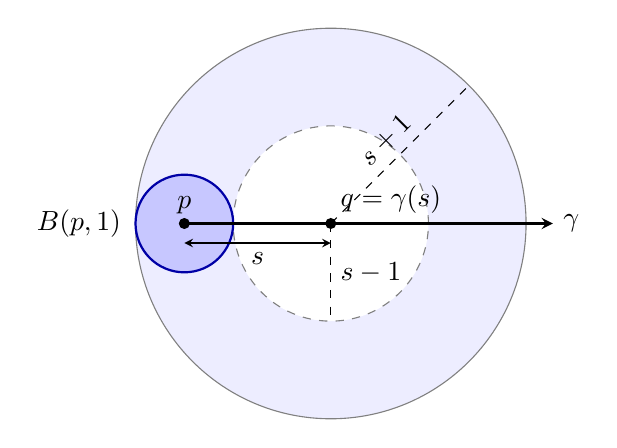
\begin{tikzpicture}[x=.62cm,y=.62cm,>=stealth]
	\fill[blue!7] (0,0) circle (4);
	\fill[white] (0,0) circle (2);
	\draw[gray] (0,0) circle (4);
	\draw[gray,dashed] (0,0) circle (2);
	\filldraw[fill=blue!22,draw=blue!65!black,thick] (-3,0) circle (1);
	\draw[thick,->] (-3,0)--(4.55,0) node[right] {\(\gamma\)};
	\draw[dashed] (0,0)--(2.828,2.828) node[midway,above,sloped] {\(s+1\)};
	\draw[dashed] (0,0)--(0,-2) node[midway,right] {\(s-1\)};
	\draw[<->] (-3,-.4)--(0,-.4) node[midway,below] {\(s\)};
	\fill (-3,0) circle (2pt) node[above] {\(p\)};
	\fill (0,0) circle (2pt) node[above right] {\(q=\gamma(s)\)};
	\node[left] at (-4.1,0) {\(B(p,1)\)};
\end{tikzpicture}

	\caption{把中心移到射线远点 \(q=\gamma(s)\) 后，固定小球落入半径 \(s-1\) 与 \(s+1\) 之间的球壳。图中的圆示意测地球，包含关系由三角不等式保证。}
	\label{g3:fig:ray-annulus}
\end{figure}

\cref{g3:fig:ray-annulus}显示了换球心的作用：小球本身未变，但容纳它的球壳厚度固定为2，相对半径却越来越小。球壳比较因此迫使大球体积随半径增长。下界的常数保留了 \(V_p(1)\)：非负 Ricci 曲率并不为单位球提供一个只依赖维数的正体积下界。例如，将平坦环面的周长缩小，\(\mathbb R\times T^{n-1}\) 的单位球体积也会变小。

\subsection{覆盖空间中的体积计数}
\label{g3:subsec:0803:02}

设 \(\pi:\widetilde M\to M\) 为万有覆盖，赋予 \(\widetilde M\) 拉回度量 \(\widetilde g=\pi^*g\)。由\cref{g3:prop:riemannian-cover-complete}，基流形完备时，覆盖空间也完备。覆盖变换群 \(\Gamma\) 的每个元素都是等距映射，因为 \(\pi\circ h=\pi\) 蕴含 \(h^*\widetilde g=\widetilde g\)。它在每条纤维上自由且传递，因而给定 \(\widetilde p\in\pi^{-1}(p)\) 后，群元素与轨道点 \(h\widetilde p\) 一一对应。

\begin{proposition}\label{g3:prop:covering-orbit-count}
	设 \((M^n,g)\) 为连通、完备、光滑无边界黎曼流形，\(\pi:(\widetilde M,\widetilde g)\to(M,g)\) 为带拉回度量的万有覆盖，\(\Gamma\) 为覆盖变换群。固定 \(\widetilde p\in\widetilde M\)。存在 \(\varepsilon>0\)，使开球族
	\[
		\{B_{\widetilde g}(h\widetilde p,\varepsilon):h\in\Gamma\}
	\]
	两两不交。记 \(v_\varepsilon=\operatorname{Vol}_{\widetilde g}B(\widetilde p,\varepsilon)\)，以及
	\[
		N_{\widetilde p}(R)
		=\#\{h\in\Gamma:
		d_{\widetilde g}(\widetilde p,h\widetilde p)\le R\}.
	\]
	则 \(0<v_\varepsilon<\infty\)，每个 \(N_{\widetilde p}(R)\) 有限，并且
	\begin{equation}\label{g3:eq:covering-volume-packing}
		N_{\widetilde p}(R)v_\varepsilon
		\le\operatorname{Vol}_{\widetilde g}B(\widetilde p,R+\varepsilon)
		\qquad(R\ge0).
	\end{equation}
	若进一步有 \(n\ge2\) 且 \(\operatorname{Ric}_g\ge0\)，则
	\begin{equation}\label{g3:eq:covering-polynomial-orbit}
		N_{\widetilde p}(R)
		\le\frac{\omega_n}{v_\varepsilon}(R+\varepsilon)^n.
	\end{equation}
\end{proposition}
\begin{proof}
	取 \(p=\pi(\widetilde p)\) 的连通均匀覆盖邻域 \(U\)，并令 \(W\) 是 \(\pi^{-1}(U)\) 中含 \(\widetilde p\) 的那一层。对任意 \(h\in\Gamma\)，集合 \(hW\) 也是一层。若 \(hW=W\)，则 \(\pi|_W\) 的单射性与 \(\pi\circ h=\pi\) 给出 \(h|_W=\mathrm{id}\)。覆盖变换由一点的像唯一确定，所以此时 \(h=\mathrm{id}\)。因此不同覆盖变换给出的层 \(hW\) 两两不交。

	距离拓扑等于流形拓扑，可以选 \(\varepsilon>0\)，使 \(B(\widetilde p,\varepsilon)\subset W\)。等距性给出
	\[
		B(h\widetilde p,\varepsilon)
		=hB(\widetilde p,\varepsilon)\subset hW,
	\]
	故这些小球两两不交，体积都等于 \(v_\varepsilon\)。光滑正体积密度保证 \(v_\varepsilon>0\)；覆盖空间完备，其闭有界球紧，故 \(v_\varepsilon<\infty\)。

	当 \(d(\widetilde p,h\widetilde p)\le R\) 时，三角不等式给出
	\[
		B(h\widetilde p,\varepsilon)
		\subset B(\widetilde p,R+\varepsilon).
	\]
	对满足此条件的任意有限个群元素，把相应小球的体积相加，所得结果不超过右侧大球的体积。后者有限而 \(v_\varepsilon>0\)，所以这样的群元素总数必然有限，并得到\eqref{g3:eq:covering-volume-packing}。

	最后，局部等距保持 Ricci 曲率及度量不等式，所以 \(\operatorname{Ric}_{\widetilde g}\ge0\)。在完备的覆盖空间上应用\cref{g3:thm:bishop-gromov}，得
	\[
		\operatorname{Vol}_{\widetilde g}B(\widetilde p,R+\varepsilon)
		\le\omega_n(R+\varepsilon)^n.
	\]
	代回即得\eqref{g3:eq:covering-polynomial-orbit}。
\end{proof}

这里计数的是覆盖空间中的轨道，右端也必须使用覆盖空间的体积。基流形中的大球会把不同提升识别为同一点，其体积通常不能替代\eqref{g3:eq:covering-volume-packing}的右端。平坦乘积的例子将显示，这一区别会改变增长的次数。

\subsection{有限生成子群的增长约束}
\label{g3:subsec:0803:03}

体积估计控制的是几何位移。为了把它用于抽象群，需选定有限个生成元，并记录至多使用多少个生成元能够到达一个元素。

\begin{definition}\label{g3:def:word-growth}
	设 \(G\) 为群，\(S\subset G\) 为有限对称生成集，即 \(S^{-1}=S\) 且 \(S\) 生成 \(G\)。元素 \(h\in G\) 的\term[zichang]{字长}[word length]定义为
	\[
		|h|_S=\min\{m\ge0:h=s_1\cdots s_m,\ s_i\in S\},
	\]
	其中空乘积表示单位元。记
	\[
		\mathcal B_S(m)=\{h\in G:|h|_S\le m\},
		\qquad \beta_S(m)=\#\mathcal B_S(m).
	\]
	若存在 \(C>0\)，使所有整数 \(m\ge0\) 都满足
	\(\beta_S(m)\le C(m+1)^d\)，则称 \(G\) 具有次数至多为 \(d\) 的\term[duoxiangshizengzhang]{多项式增长}[polynomial growth]。
\end{definition}

这一性质不依赖有限生成集的选择。事实上，若 \(T\) 是另一有限对称生成集，取
\[
	A=\max\bigl(\{1\}\cup\{|s|_T:s\in S\}\bigr),
\]
把每个 \(S\) 中的字母换成至多 \(A\) 个 \(T\) 中的字母，便得到
\(\mathcal B_S(m)\subset\mathcal B_T(Am)\)。交换 \(S,T\) 得到反向的线性尺度比较。因此，多项式上界的次数可以保持，常数则随生成集变化。

\begin{theorem}\label{g3:thm:fundamental-subgroup-growth}
	设 \((M^n,g)\) 为连通、完备、光滑无边界黎曼流形，\(n\ge2\)，且 \(\operatorname{Ric}\ge0\)。则 \(\pi_1(M,p)\) 的每个有限生成子群 \(G\)，相对于任意有限对称生成集 \(S\)，都满足
	\[
		\beta_S(m)\le C_S(m+1)^n
		\qquad(m=0,1,2,\ldots),
	\]
	其中 \(C_S\) 可以依赖流形、基点、子群和生成集。
\end{theorem}
\begin{proof}
	利用万有覆盖的覆盖变换群与基本群的同构，将 \(G\) 看成覆盖变换群 \(\Gamma\) 的子群。选定 \(\widetilde p\in\pi^{-1}(p)\)。若 \(G\) 为平凡群，结论由 \(\beta_S(m)=1\) 得到；以下设 \(G\) 非平凡，并在生成集中删去单位元。令
	\[
		L=\max_{s\in S}d_{\widetilde g}(\widetilde p,s\widetilde p)>0.
	\]
	覆盖变换等距，因此任意 \(g,h\in\Gamma\) 满足
	\[
		d(\widetilde p,gh\widetilde p)
		\le d(\widetilde p,g\widetilde p)
		+d(g\widetilde p,gh\widetilde p)
		=d(\widetilde p,g\widetilde p)
		+d(\widetilde p,h\widetilde p).
	\]
	反复应用可知，若 \(|h|_S\le m\)，则
	\(d(\widetilde p,h\widetilde p)\le mL\)。不同群元素作用于 \(\widetilde p\) 得到不同点，所以
	\[
		\beta_S(m)\le N_{\widetilde p}(mL).
	\]
	应用\cref{g3:prop:covering-orbit-count}，得到
	\[
		\beta_S(m)
		\le\frac{\omega_n}{v_\varepsilon}(mL+\varepsilon)^n
		\le\frac{\omega_n(L+\varepsilon)^n}{v_\varepsilon}(m+1)^n.
	\]
	取最后一个系数为 \(C_S\) 即可。
\end{proof}

定理的量词逐个作用于有限生成子群。证明中，有限生成性恰好用于取得生成元位移的有限上界 \(L\)；所得估计本身没有给出整个基本群的一组有限生成元。另一个直接用途是排除增长过快的子群。例如，自由群 \(F_2=\langle a,b\rangle\) 相对于 \(\{a,a^{-1},b,b^{-1}\}\)，长度恰为 \(m\ge1\) 的约化字有 \(4\cdot3^{m-1}\) 个：第一个字母有四种选择，此后每次排除前一字母的逆元，尚有三种选择。因此 \(F_2\) 不可能作为上述基本群的子群。

\subsection{Euclid、双曲及乘积模型}
\label{g3:subsec:0803:04}

模型计算同时检验小尺度和大尺度。光滑 \(n\) 维度量的小球都有 \(n\) 维 Euclid 主项；大球则会反映曲率累积以及紧方向被填满之后的变化。

\begin{example}\label{g3:exm:euclidean-hyperbolic-volume-growth}
	在 Euclid 空间 \(\mathbb R^n\) 中，
	\[
		V_p(R)=\omega_nR^n
	\]
	对所有 \(R>0\) 成立。对曲率为 \(-a^2\) 的双曲模型，取 \(a>0\)、\(n\ge2\)，其全局极坐标度量为
	\[
		g=\mathrm dr^2+
		\left(\frac{\sinh(ar)}a\right)^2g_{S^{n-1}}.
	\]
	这里全局坐标可由双曲面
	\[
		-x_0^2+|x|^2=-a^{-2},\qquad x_0>0
	\]
	上的参数式
	\[
		x_0=a^{-1}\cosh(ar),\qquad
		x=a^{-1}\sinh(ar)u,\qquad u\in S^{n-1},
	\]
	直接得到：将其微分代入 \(-\mathrm dx_0^2+|\mathrm dx|^2\)，径向项为 \(\mathrm dr^2\)，角向项为 \((\sinh(ar)/a)^2g_{S^{n-1}}\)，交叉项为零。每条从中心到半径 \(r\) 的曲线长度至少为 \(r\)，因为离开中心后其速度长度不小于径向速度的绝对值；径向曲线达到此下界。故坐标半径就是中心距离，球体积为
	\begin{equation}\label{g3:eq:hyperbolic-volume-growth}
		V_{-a^2,n}(R)
		=\frac{\sigma_{n-1}}{a^{n-1}}
		\int_0^R\sinh(at)^{n-1}\,\mathrm dt.
	\end{equation}
	当 \(R\downarrow0\) 时，\(\sinh(at)/a=t+O(t^3)\)，所以
	\[
		V_{-a^2,n}(R)=\omega_nR^n\bigl(1+O(R^2)\bigr).
	\]
	当 \(R\to\infty\) 时，
	\[
		\sinh(aR)^{n-1}
		\sim 2^{-(n-1)}e^{(n-1)aR}.
	\]
	将积分与 \(e^{(n-1)aR}\) 的比求极限，或对这个渐近式积分，得到
	\begin{equation}\label{g3:eq:hyperbolic-volume-asymptotic}
		V_{-a^2,n}(R)
		\sim
		\frac{\sigma_{n-1}}{2^{n-1}(n-1)a^n}
		e^{(n-1)aR}.
	\end{equation}
	例如 \(n=2\) 时可直接积分：
	\[
		V_{-a^2,2}(R)=\frac{2\pi}{a^2}\bigl(\cosh(aR)-1\bigr).
	\]
	这里的指数增长说明，非负 Ricci 假设对多项式体积上界具有实质作用。
\end{example}

\begin{example}\label{g3:exm:flat-product-volume-growth}
	设 \(a,b\ge1\) 为整数，\(T^b=\mathbb R^b/\Lambda\) 为平坦环面，赋予
	\[
		M=\mathbb R^a\times T^b
	\]
	乘积度量。其总维数为 \(n=a+b\)，曲率恒为零。记环面直径为 \(D>0\)、体积为 \(v_T>0\)，固定中心 \((0,y_0)\)。

	先核对距离。任意从 \((0,y_0)\) 到 \((x,y)\) 的分片光滑曲线 \((\alpha,\beta)\) 都满足
	\[
		\int\sqrt{|\dot\alpha|^2+|\dot\beta|^2}
		\ge
		\sqrt{\left(\int|\dot\alpha|\right)^2+
		\left(\int|\dot\beta|\right)^2}
		\ge\sqrt{|x|^2+d_T(y_0,y)^2}.
	\]
	第一个不等式是对向量值函数
	\((|\dot\alpha|,|\dot\beta|)\) 的积分三角不等式。反过来，分别取两个因子中的最短线，并将它们参数化在 \([0,1]\) 上，使速度长度恒为各自端点距离，便达到下界。因此
	\[
		d_M((0,y_0),(x,y))^2=|x|^2+d_T(y_0,y)^2.
	\]
	两个因子均完备，距离公式又说明乘积中的 Cauchy 序列逐分量收敛，所以 \(M\) 完备。

	用乘积体积密度逐纤维积分，可得对所有 \(R>0\) 都成立的精确公式
	\begin{equation}\label{g3:eq:flat-product-volume-formula}
		V_{(0,y_0)}(R)
		=\omega_a\int_{T^b}
		\bigl(R^2-d_T(y_0,y)^2\bigr)_+^{a/2}\,\mu_T(y),
	\end{equation}
	其中 \(s_+=\max\{s,0\}\)。因为 \(0\le d_T(y_0,y)\le D\)，当 \(R>D\) 时，
	\begin{equation}\label{g3:eq:flat-product-volume-bounds}
		\omega_av_T(R^2-D^2)^{a/2}
		\le V_{(0,y_0)}(R)
		\le\omega_av_TR^a.
	\end{equation}
	特别地，对 \(R\ge2D\)，有
	\[
		\left(\frac34\right)^{a/2}\omega_av_TR^a
		\le V_{(0,y_0)}(R)
		\le\omega_av_TR^a,
	\]
	而令 \(R\to\infty\) 得到
	\[
		V_{(0,y_0)}(R)\sim\omega_av_TR^a.
	\]

	小尺度却仍是 \(n=a+b\) 维的。设
	\(\rho=\frac12\min_{\lambda\in\Lambda\setminus\{0\}}|\lambda|>0\)。
	当 \(0<R<\rho\) 时，覆盖映射
	\(\mathbb R^{a+b}\to\mathbb R^a\times T^b\)
	在 Euclid 半径 \(R\) 的球上限制为到上述球的微分同胚，并保持黎曼度量：任意 \(y\) 的最短代表可由使 \(|\widetilde y+\lambda|\) 最小的格点给出，距离公式保证满射；两个球内点若相差非零格向量，其距离小于 \(2R<2\rho\)，又与格向量长度下界矛盾。因此
	\[
		V_{(0,y_0)}(R)=\omega_{a+b}R^{a+b}
		\qquad(0<R<\rho).
	\]
	公式\eqref{g3:eq:flat-product-volume-formula}描述了从小尺度到大尺度的整个过渡。当 \(a=1\) 时，大球体积恰为线性量级，说明\cref{g3:thm:noncompact-volume-growth}的线性下界在一般情形下不能提高到更大的幂次。
\end{example}

上述乘积的万有覆盖是 \(\mathbb R^{a+b}\)，覆盖变换沿环面因子的格点作平移。因此，基流形的大球按 \(R^a\) 增长，覆盖空间的大球却按 \(R^{a+b}\) 增长。覆盖体积计数使用后一个增长率，正是因为它需要把所有不同提升的小球分别容纳进去。
% 纲要条目排为编号小节标题，并进入目录与书签；说明段仍保留于纲要注释中。
